\documentclass[a4paper,11pt]{article}
\usepackage{graphicx}
\usepackage{amsmath}
\usepackage{hyperref}
\usepackage{geometry}
\usepackage{natbib}
\usepackage{project}
\usepackage{tikz}
\usetikzlibrary{positioning, shapes.geometric, arrows}
\setlength{\headheight}{13.6pt}

\begin{document}

\section{Introduction}
The analysis investigates the relationship between neighborhood poverty levels and school enrollment across different U.S. regions. By combining datasets, my aim is to uncover patterns that indicate educational inequalities driven by socioeconomic factors.

We focus on:
    \begin{itemize}
        \item How does neighborhood poverty correlate with school enrollment rates in the US?
    
        \item Regional disparities in poverty and their potential implications for educational equality?
    \end{itemize}

\section{Data}
    \subsection{Data Sources}
        \begin{itemize}
            \item \textbf{Dataset 1: School Neighborhood Poverty Estimates 2020-2021}
            This data set from the National Center for Education Statistics \(\text(NCES)\) includes data on neighborhood poverty levels surrounding schools, which can serve as a proxy for educational access and socioeconomic conditions of the community. \cite{dataset1}

            \item \textbf{Dataset 2: Report Card Enrollment}

            This data set provides detailed school enrollment statistics disaggregated by school, district, and state for the 2022-23 school year. It includes student counts by demographics, which can help analyze how regional poverty levels could influence enrollment and highlight disparities between regions. \cite{dataset2}
        \end{itemize}

    \subsection{Data Pipeline}
        The data pipeline engineering is designed and developed with Python has three main modules: extractor, transform, and loader each module contains respective functionalities. Furthermore, the pipeline helper has the responsibility to initialize the desired configuration for data sources.

        After configuration Initialization for data sources, each module performs its responsibility. First \texttt{extract} from extractor module is used to extract the data source from url, second \texttt{delete\_columns} from transform module deletes the list of useless columns specified for every dataset. Additionally, eliminate the rows contain null or empty records, once all the transformations have been applied, the data set is then loaded into the sqlite database using \texttt{load\_df\_to\_sqlite} from loader module.

        \begin{figure}[h]
            \centering
            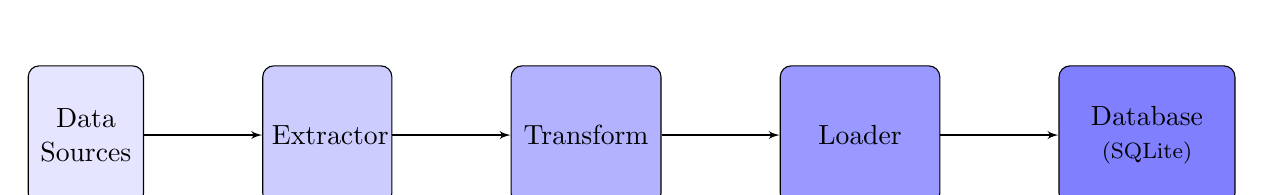
\begin{tikzpicture}[node distance=1cm and 1.5cm, auto]
                \tikzstyle{datasource} = [rectangle, draw, fill=blue!10,
                text width=3.5em, text centered, rounded corners, minimum height=5em]
            \tikzstyle{E} = [rectangle, draw, fill=blue!20,
                text width=4em, text centered, rounded corners, minimum height=5em]
            \tikzstyle{T} = [rectangle, draw, fill=blue!30,
                text width=4.75em, text centered, rounded corners, minimum height=5em]
            \tikzstyle{L} = [rectangle, draw, fill=blue!40,
                text width=5.1em, text centered, rounded corners, minimum height=5em]
            \tikzstyle{db} = [rectangle, draw, fill=blue!50,
                text width=6em, text centered, rounded corners, minimum height=5em]
            \tikzstyle{line} = [draw, -latex', shorten >=0pt, shorten <=0pt]

            \node [datasource] (source) {Data Sources \\ \footnotesize};
            \node [E, right=of source] (extractor) {Extractor};
            \node [T, right=of extractor] (transform) {Transform};
            \node [L, right=of transform] (loader) {Loader};
            \node [db, right=of loader, text width=2cm, align=center] (database) {Database \\ \footnotesize (SQLite)};

            \path [line] (source) -- (extractor);
            \path [line] (extractor) -- (transform);
            \path [line] (transform) -- (loader);
            \path [line] (loader) -- (database);
        \end{tikzpicture}
    \caption{ETL Pipeline Flow}
    \label{fig:etl}
    \end{figure}
    
    \subsection{Data Pipeline Output}
    
        \begin{itemize}
            \item \textbf{School Neighborhood Poverty Estimates 2020-2021:}
             The data is organized with geospatial data (latitude and longitude) defining the locations of various education systems. It also includes the income-to-poverty ratio (IPR) which measure the socioeconomics conditions in surroundings to the schools. Additionally, It defines the standard error of the IPR for each area.
            \begin{figure}[ht!]
                \centering
                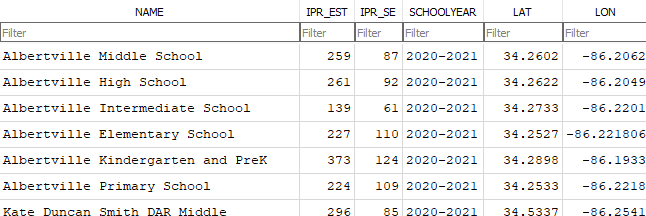
\includegraphics[width=0.9\textwidth]{images/SchoolNeighborhoodPovertyData.png}
                \caption{School neighborhood poverty estimate 2020-2021 dataset}
                \label{fig:dataset1}
            \end{figure}
            
           
            
\newpage
            \item \textbf{Report Card Enrollment:} The data is structured for analyzing school-specific or regional educational trends. Mainly it contains the statistical metrics of enrollment in different Education system. Also, providing the income category by which students are belonging. 
            \begin{figure}[h!]
                \centering
                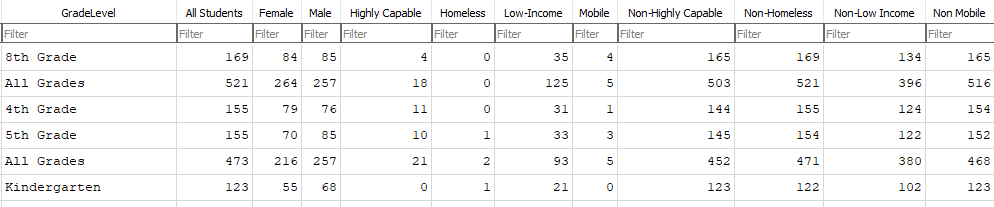
\includegraphics[width=0.9\linewidth]{images/ReportCardEnrollmentData.png}
                \caption{Report card Enrollment}
                \label{fig:dataset2}
            \end{figure}
        \end{itemize} 

    \subsection{Licenses and Permissions} The datasets I finalized have open licenses allowing public use and redistribution. School Neighborhood Poverty Estimates (2020-21) dataset is licensed under the CC BY 4.0 license (Creative Commons Attribution 4.0 International License). This license allows public to share and adapt the data, provided that appropriate credit is given, and any derived works are shared under the same license.
    Common Core of Data (CCD) - School Nonfiscal Data Files and Documentation, 2018-19 dataset is also licensed under the CC BY 4.0 license. This similarly allows public use, distribution, and modification as long as proper attribution is given.

    Therefore, data for this project are licensed under the Open Licenses and Creative Commons Attribution 4.0 International (CC BY 4.0) license. For more information, visit \href{https://creativecommons.org/licenses/by/4.0/}CC BY 4.0 License and \href{https://resources.data.gov/open-licenses/}Open Licenses

\vspace{0.2cm}

\section{Analysis}

The data pipeline was used to import and perform the data engineering tasks before the analysis was started. The analysis was started with exploring each dataset individually and by doing so found few very exciting insights. The conducted analysis revealed insights on how poverty level, represented as IPR-EST (Income-to-Poverty Ratio Estimate) relates to school enrollment rates. The neighborhood poverty conditions play a vital role in school enrollment lower income (with less IPR) have lesser school enrollment and this might be incfluenced by different socio-economic factors such as lack of resources, social stigma, instability of residence meaning frequent relocations which disturb education.

\begin{figure}[ht!]
    \centering
    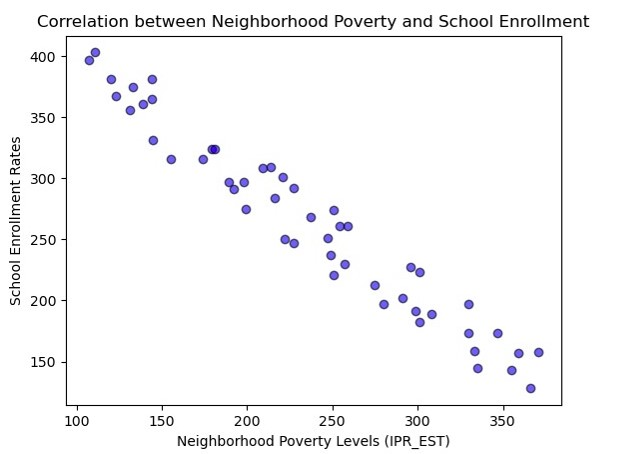
\includegraphics[width=0.6\textwidth]{images/Comparitive-Analysis.png}
    \caption{Comparative Analysis}
    \label{fig:temp_change}
\end{figure}

Furthermore, the data is categorized into different regions in the US to help in a clear regional analysis. Fig. 5 highlights the disparities in poverty levels across different regions in the USA. South region shows highest IPR ES value reaching up to 350 while lowest poverty records are found in West region up to 180.Varying poverty levels create a distinction in the society, meaning regions with better infrastructure or higher job opportunities have better education systems while other regions, for e.g South USA in our case, could have lesser school enrollments which would also mean children from poorer regions receive lesser to no education and this education is of lower standard as compared to regions with a greater number of schools and better resources.
This inequality can perpetuate a cycle where children below poverty line will be deprived of good education and will have lesser number of opportunities in future. Poverty reduces chances of fair education which greatly impacts future of the children and deepens regional economics disparity. 

\begin{figure}[h]
    \centering
    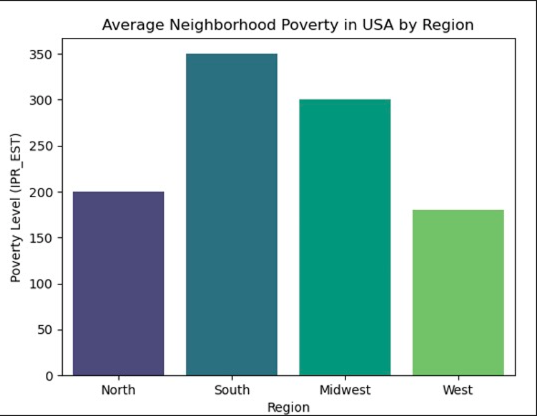
\includegraphics[width=0.6\textwidth]{images/Regional-Analysis.png}
    \caption{Regional Analysis}
    \label{fig:sea_levels}
\end{figure}
\vspace{10cm}


\section*{Conclusions}

The study identifies a clear correlation between neighborhood poverty levels and school enrollment rates, revealing that areas with lower Income-to-Poverty Ratio Estimates (IPR-EST) tend to experience reduced school enrollment. Additionally, regional disparities across the four different regions of the United States highlight significant inequities in access to quality education. This imbalance contributes to unequal opportunities and has far-reaching implications for the development and growth of the affected regions within the United States.


\bibliographystyle{plain}
\bibliography{reference}
\end{document}